%%%%%%%%%%%%%%%%%%%%%%%%%%%%%%%%%%%%%%%%%%%%%%%%%%%%%%%%%
% Niniejszy plik przedstawia przykładowy skład 
% pracy dyplomowej na Wydziale Matematyki PWr. 
% 
% Autorzy: 
% Damian Fafuła
% Michał Kijaczko
% Jakub Michalczak
% Maciej Miśta
% Dagmara Nowak
% Tomasz Skalski
% Wojciech Słomian
%
%% Data utworzenia: 8.05.2018
% Numer wersji: 1
%
% Poniższą formatkę można rozpowszechniać i edytować 
% pod warunkiem zachowania numeru wersji, 
% informacji o autorach i dodaniu informacji 
% o wprowadzonych zmianach.
%
%%%%%%%%%%%%%%%%%%%%%%%%%%%%%%%%%%%%%%%%%%%%%%%%%%%%%%%%%
% Domyślną opcją jest: praca magisterska, język polski.
% W przypadku pracy pisanej w języku angielskim dodajemy 
% opcję [english].
% Dla pracy licencjackiej dodajemy opcję [licencjacka].
% Dla pracy inżynierskiej dodajemy opcję [inzynierska].
% Dopuszczalne są podwójne opcje, np. [licencjacka, english].
% Opcje dodajemy w kwadratowym nawiasie przy \documentclass.
%
%
%%%%%%%%%%%%%%%%%%%%%%%%%%%%%%%%%%%%%%%%%%%%%%%%%%%%%%%%%
\documentclass[inzynierska]{pwr_wmat_praca_dyplomowa}
%%%%%%%%%%%%%%%%%%%%%%%%%%%%%%%%%%%%%%%%%%%%%%%%%%%%%%%%%
%              DANE DO PRACY
%
% W przypadku pracy dyplomowej w języku angielskim nie jest konieczne 
% wypełnianie pól: \tytul{}, \kierunek{}, \specjalnosc{}, 
%                  \streszczenie{}, \slowakluczowe{}.
%%%%%%%%%%%%%%%%%%%%%%%%%%%%%%%%%%%%%%%%%%%%%%%%%%%%%%%%%
%
% Imię i nazwisko autora
\autor{Aleksander Jakóbczyk}
%
% Tytuł pracy dyplomowej 
\tytul{Zastosowanie stochastycznej
	optymalizacji do gier
	częściowo obserwowalnych} 
\tytulang{Tytuł pracy dyplomowej w języku angielskim}
%
% Tytuł / stopień / imię i nazwisko opiekuna
\opiekun{dr inż. Andrzej Giniewicz}
%
% Kierunek studiów wybieramy spośród następujących:
% 1) Matematyka
% 2) Matematyka i Statystyka
% 3) Matematyka stosowana
\kierunekstudiow{Matematyka stosowana}
%
% Kierunek studiów po angielsku wybieramy spośród następujących:
% 1) Mathematics
% 2) Mathematics and Statistics
% 3) Applied Mathematics
\kierunekstudiowang{Mathematics}
%
% Specjalność wybieramy spośród następujących: 
% KIERUNEK: Matematyka
% 1) Matematyka teoretyczna,
% 2) Statystyka matematyczna,
% 3) Matematyka finansowa i ubezpieczeniowa,
%
% KIERUNEK: Matematyka i Statystyka
% 4) Matematyka,
% 5) Statystyka i analiza danych, 
%
% 6) -- (w przypadku braku specjalizacji).
\specjalnosc{--} 
%
% Specjalność w języku angielskim wybieramy spośród następujących:
% KIERUNEK: Matematyka
% 1) Theoretical Mathematics,
% 2) Mathematical Statistics,
% 3) Financial and Actuarial Mathematics,
%
% KIERUNEK: Matematyka i Statystyka
% 4) Mathematics,
% 5) Statistics and Data Analysis,
%
% KIERUNEK: Applied Mathematics
% 6) Financial and Actuarial Mathematics, 
% 7) Mathematics for Industry and Commerce,
% 8) Computational Mathematics,
% 9) Modelling, Simulation and Optimization.
%
% 10) -- (w przypadku braku specjalizacji).
\specjalnoscang{Theoretical Mathematics} 
%
% Krótkie streszczenia po polsku i angielsku
% - nie dłuższe niż 530 znaków.
\streszczenie{Celem rozprawy jest wyznaczenie nieoczekiwanych strategii w grach częściowo obserwowalnych za pomocą metod
	stochastycznej optymalizacji. Praca będzie opierać się na wynikach Cauwet i Teytauda z 2018 roku, w których
	przedstawili nieoczekiwane strategie dla kilku klasycznych gier oraz kilku metod optymalizacji. Podjęta zostanie
	próba odtworzenia oraz rozszerzenia wyników na kolejną grę. Przeprowadzona zostanie analiza porównawcza dla
	różnych metod optymalizacji.}
\streszczenieang{Tutaj piszemy krótkie streszczenie pracy w języku angielskim (nie powinno być dłuższe niż 530 znaków).}
%
% Podajemy najważniejsze słowa kluczowe po polsku i angielsku
% - w obu przypadkach, nie więcej niż 150 znaków.
\slowakluczowe{tutaj podajemy najważniejsze słowa kluczowe (łącznie nie powinny być dłuższe niż 150 znaków).}  
\slowakluczoweang{tutaj podajemy najważniejsze słowa kluczowe w języku angielskim (łącznie nie powinny być dłuższe niż 150 znaków)}
%
%
%%%%%%%%%%%%%%%%%%%%%%%%%%%%%%%%%%%%%%%%%%%%%%%%%%%%%%%%%
% Definicje, lematy, twierdzenia, przykłady i wnioski
% Komendy wywołujące twierdzenia, definicje, itd., 
% czyli 'theorem', 'definition', 'corollary', itd., 
% można zmienić wedle uznania.
\theoremstyle{plain}
\newtheorem{theorem}{Twierdzenie}
\numberwithin{theorem}{chapter}
\newtheorem{lemma}[theorem]{Lemat} 
\newtheorem{corollary}[theorem]{Wniosek}
\newtheorem{fact}[theorem]{Fakt}
\theoremstyle{definition}
\numberwithin{theorem}{chapter}
\newtheorem{definition}[theorem]{Definicja} 
\newtheorem{example}[theorem]{Przykład}
\newtheorem{note}[theorem]{Uwaga}
%%%%%%%%%%%%%%%%%%%%%%%%%%%%%%%%%%%%%%%%%%%%%%%%%%%%%%%%%

\usepackage{amsmath}
\usepackage{amsthm}
\usepackage{amsfonts}
\usepackage{amssymb}
\usepackage{graphicx}
\usepackage{caption}
\usepackage{xcolor}
\usepackage{algpseudocode,algorithm,algorithmicx}
\usepackage{enumitem}
\usepackage[plmath]{polski}
\usepackage{booktabs}

%icomma
\DeclareRobustCommand{\bbone}{\text{\usefont{U}{bbold}{m}{n}1}}
\DeclareMathOperator{\EX}{\mathbb{E}}% expected value
\DeclareCaptionLabelFormat{custom2}
{%
	#1 \thealgorithm:
}

%%%%%%%%%%%%%%%%%%%%%%%%%%%%%%%%%%%%%%%%%%%%%%%%%%%%%%%%%
%%%%%%%%%%%%%%%%%%%%%%%%%%%%%%%%%%%%%%%%%%%%%%%%%%%%%%%%%
\begin{document}
\frontmatter
\maketitle
\mainmatter
\tableofcontents
%\listoffigures
%\listoftables

{\backmatter \chapter{Wstęp}}
%We wstępie zapowiadamy, o czym będzie praca. Próbujemy zachęcić czytelnika do dalszej lektury, np. krótko informując, dlaczego wybraliśmy właśnie ten temat i co nas w nim zainteresowało.

%\chapter{Rozdział pierwszy}
%Tabela \ref{tab:przykladowa} przedstawia przykładową tabelę. Do tworzenia tabeli służą m.in. środowiska \texttt{tabular} oraz \texttt{table}. Istnieje możliwość numeracji dwustopniowej, gdzie pierwsza cyfra oznacza numer rozdziału, a druga – kolejny numer tabeli w tym rozdziale. Tytuł powinien znajdować się centralnie nad tabelą, $12$ pkt odstępu od tekstu zasadniczego nad i pod tabelą wraz z tytułem. Jeśli tabela jest cytowana – należy podać centralnie pod tabelą źródło jej pochodzenia, np. opracowanie własne, opracowano na podstawie danych z GUS.
%\begin{table}[ht]
%\caption{Podstawowa Tabela}
%\centering
%\begin{tabular}{ccc}
%\hline
%\hline                       
%Państwo & PKB (w milionach USD )& Stopa bezrobocia  \\  [0.5ex] 
%\hline 
%Stany Zjednoczone & 75 278 049 & 4,60\%  \\
%Chiny & 11 218 281 & 4,10\%   \\
%Japonia & 4 938 644 & 3,10\%  \\
%Niemcy & 3 466 639 & 6,00\%   \\
%Wielka Brytania & 2 629 188 & 4,60\%  \\ [1ex]  
%\hline 
%\end{tabular}
%\caption*{\textit{Źródło: opracowanie własne}}
%\label{tab:przykladowa} 
%\end{table}
%
%%Do cytowania używamy komendy \texttt{cite}. W nawiasie klamrowym podajemy klucz, którego użyliśmy w pliku \emph{bibliografia.bib}. Przykład: \cite{einstein} lub \cite[chap. 2]{latexcompanion}.
%
%\section{Podrozdział pierwszy}
%
%\begin{table}[H]
%\caption{Podstawowa Tabela}
%\centering
%\begin{tabular}{ccc}
%\hline
%\hline                       
%Państwo & PKB (w milionach USD )& Stopa bezrobocia  \\  [0.5ex] 
%\hline 
%Stany Zjednoczone & 75 278 049 & 4,60\%  \\
%Chiny & 11 218 281 & 4,10\%   \\
%Japonia & 4 938 644 & 3,10\%  \\
%Niemcy & 3 466 639 & 6,00\%   \\
%Wielka Brytania & 2 629 188 & 4,60\%  \\ [1ex]  
%\hline 
%\end{tabular}
%\caption*{\textit{Źródło: opracowanie własne}}
%\label{tab:przykladowa2} 
%\end{table}
%
%\section{Podrozdział drugi}
%
%Rysunki do pracy dyplomowej należy wstawiać w sposób podobny do wstawiania tabel, z~zasadniczą różnicą polegającą na tym, że podpis powinno umieszczać się centralnie pod rysunkiem, a nie powyżej niego. Numeracja i sposób cytowania pozostają bez zmian, przy czym tabele i rysunki nie mają numeracji wspólnej, np. po Tabeli \ref{tab:przykladowa2} występuje Rysunek \ref{rys1} (o ile jest to pierwszy rysunek rozdziału pierwszego), a nie Rysunek $1.3$.
%
%\begin{figure}[ht]
%
%\centering
%                     
%
\includegraphics[scale=0.27]{logo_w13.jpg}
%\caption{Podstawowy Rysunek}\label{rys1}
%\end{figure}
%\label{rys:przykladowy} 


\chapter{Definicje, lematy, twierdzenia, przykłady i wnioski}
Celem algorytmów, które będziemy wykorzystywać, jest znalezienie optymalnej strategii dla graczy w dwuosobowych grach częściowo obserwowalnych. Aby matematycznie opisać pojęcia gry i strategii optymalnej, wprowadzimy kilka podstawowych definicji.
Definicje dotyczące podstaw teorii gier pochodzą z prac \cite{platkowski2012wstkep},\cite{prisner2014game}.

\section{Czym jest gra?}
Omówmy zatem co nazywamy gra w matematyce.

Gra w matematycznej teorii gie to sytuacja, w której gracze wybierają swoje strategie i otrzymują nagrody lub kary w zależności od podjętych decyzji  oraz losowych zdarzeń. Teoria gier pozwala na modelowanie i analizowanie takich sytuacji oraz umożliwia znajdowanie rozwiązań, które są optymalne dla graczy.

Matematyczna definicja gry w teorii gier zazwyczaj zaczyna się od określenia następujących elementów:

\begin{itemize}
	\item Zbioru graczy: Zbiór graczy to zbiór wszystkich graczy biorących udział w grze. Może to być zbiór składający się z dwóch lub więcej elementów, w zależności od typu gry.
	
	\item Zbioru strategii: Zbiór strategii to zbiór wszystkich możliwych strategii, które mogą być wybierane przez graczy. Strategia to plan działania gracza, który zakłada, jakie ruchy gracz zamierza podjąć w danej grze.
	
	\item Funkcji zwrotu: Funkcja zwrotu określa nagrody lub kary, które gracze otrzymują w zależności od ich strategii i losowych zdarzeń.
	
	\item Struktury informacji: Struktura informacji określa, jakie informacje są dostępne dla graczy w momencie podejmowania decyzji. Informacje mogą być pełne lub częściowe, co wpływa na możliwe strategie graczy i ich skuteczność.
\end{itemize}

Gry mogą być podzielone na kilka kategorii w zależności od kilku różnych kryteriów. Jednym z takich kryteriów jest moment, w którym gracze podejmują decyzje:
%\begin{definition}[Gra]
%Gra w matematycznym sensie jest sytuacja, w której gracze podejmują  decyzje zgodnie z określonymi zasadami w celu uzyskania jakiejś wypłaty.
%\end{definition}
\begin{definition}[Gra w postaci strategicznej]
Jest to typ gry, w której gracze podejmują decyzje w tym samym
momencie.
\end{definition}
\begin{definition}[Gra w postaci ekstensywnej]
	Jest to typ gry, w której gracze podejmują decyzje we wcześniej
	ustalonej kolejności.
\end{definition}
Przykładami gier w postaci strategicznej są gry kamień papier nożyce, oszust czy też mora. Natomiast przykładami gier w postaci ekstensywnej są szachy, warcaby oraz go.

Gry możemy również dzielić ze względu na posiadaną wiedzę.
\begin{definition}[Gra z kompletną informacją]
	Jest to typ gry, w której gracze mają informacje o możliwych
	przyszłych wynikach gry i o zbiorach możliwych strategii.
\end{definition}
\begin{definition}[Gra częściowo obserwowalna]
	Jest to przeciwnie gier z kompletną informacją.
\end{definition}
Przykładami gier z kompletną informacją są szachy, warcaby oraz go.
Natomiast przykładami gier częściowo obserwowanymi są wszelkie gry posiadające w rozgrywce pewien elementy losowe takie jak rzut kostką czy też dobieranie kart. 

Istnieje jeszcze wiele innych podziałów gier ze wglądu na kategorie takie jak liczba graczy,zbiory dostępnych akcji, możliwość tworzenia koalicji i wiele innych.

\section{Definicje i Oznaczenia}
\subsection{Strategie proste}
Wprowadźmy podstawowe oznaczenia potrzebne nam do tego, aby móc zdefiniować czym jest strategia optymalna.
\begin{itemize}
	\item $ N = \{1,2,\dots, n\} $ -- zbiór graczy,
	\item $A_i,\; i \in N $ -- niepusty zbiór strategii  czystych gracza $i$,
	\item $m_i = |A_i|$ -- liczba strategi gracza $i$,
	\item $A = \displaystyle\prod_{i \in N} A_i$ -- zbiór wszystkich strategii gry, 
	\item $u_i : A \rightarrow \mathbb{R} $ -- funkcja wypłaty gracza $i$,
	\item $a=(a_1,a_2,\dots,a_n)=(a_i)_{i \in N},\; a_i \in A_i$ -- profil gry w strategiach czystych,
	\item $u_i(a) = u_i(a,a_{-i})$ -- wypłata gracza $i$ z profilu $a$,
	\item $a_{-i} = (a_i)_{i\in N \setminus \{i\}}$, -- profil wszystkich strategii poza strategią graca $i$.
\end{itemize}
	\begin{definition}[Gra strategiczna]
		Grą strategiczną nazywamy trójkę $GS = \langle N, (A_i)_{i \in N},(u_i)_{i \in N} \rangle $.
	\end{definition}
	
	\begin{definition}[Równowaga Nasha w strategiach czystych gry strategicznej]
		Równowaga Nasha w strategiach czystych gry strategicznej jest to profil gry $a^*= (a_1^*,a_2^*,\dots,a_N^*)\in A$, takim, że
		\begin{align*}
			\mathop{\forall}{i \in N}\;
			\mathop{\forall}{a_i \in A_i} \quad
			u_i(a_i^*,a_{-i}^*) \ge u_i(a_i, a_{-i}^*).
		\end{align*}
	\end{definition}
	Zatem jest to profil gry, w którym istnieje strategia czysta dająca nie gorsze wyniki od dowolnej innej strategii czystej.
	Okazuje się jednak, że taki stan nie zawsze istnieje w strategiach czystych, np. w grze kamień papier nożyce strategia grania tylko kamienia daje gorsze rezultat przeciwko graniu tylko papieru. Podobnie ze strategią grania tylko nożyc i grania tylko papieru.
	\subsection{Strategie mieszane}
	%zmien sigmy na alfy
	\begin{definition}[Strategia mieszana]
		Strategia mieszana $\sigma_i$ graca $i$ w grze strategicznej $GS = \langle N, (A_i)_{i \in N},(u_i)_{i \in N} \rangle $. Nazywamy rozkład prawdopodobieństwa na zbiorze strategi czystych $A_i$:
		\begin{align*}
			\sigma_i = (\sigma_{i1}, \sigma_{i2},\dots,\sigma_{im_i})
		\end{align*}
	gdzie $\sigma_{ik}$ oznacza prawdopodobieństwo, że gracz $i$ zagra strategie czysta $k\in A_i$.  
	\end{definition}

	\begin{fact}
		Strategia czysta jest szczególnym przypadkiem strategij mieszanej, w którym prawdopodobieństwo zagrania jednej z dostępnych strategii wynosi 1.
	\end{fact}
	Wprowadźmy dodatkowe oznaczenia:
 	\begin{itemize}
 		\item $\Sigma_i  = \left\{ \sigma_i: A_i \rightarrow [0,1],\displaystyle\sum_{k=1}^{n} \sigma_{ik} = 1, \sigma_{ki}\ge 0 \right\}$ -- zbiór strategii mieszanych gracza $i$,
 		\item  $\sigma = (\sigma_1, \sigma_2,\dots,\sigma_n)$ -- profil gry,
 		\item $u_i(\sigma) = u_i(\sigma_i,\sigma_{-i})$ -- wypłata gracza $i$ z profilu $\sigma$,
 		\item $\sigma_{-i} = (\sigma_i)_{i\in N \setminus \{i\}}$, -- profil wszystkich strategii poza strategią graca $i$. 
 	\end{itemize}
	\begin{definition}[Równowaga Nasha w strategiach mieszanej gry strategicznej]
		Profil gry strategicznej $\sigma_i^*$ jest Równowagą Nasha gdy:
		\begin{equation*}
			\mathop{\forall}{i \in N}\;
			\mathop{\forall}{\sigma_i \in \Sigma_i} \quad
			u_i(\sigma_i^*,\sigma_{-i}^*) \ge u_i(\sigma_i, \sigma_{-i}^*)
		\end{equation*}
	Równowaga Nasha interpretujemy jako taki profil gry, w którym żaden z graczy nie opłaca się zmieniać swojej strategi, ponieważ nie skutkuje to zwiększeniem swoich zysków.
	\end{definition}

	\section{Twierdzenia}
	Algorytmy \ref{alg:LEBR}, \ref{alg:ILEBR 1}, \ref{alg:ILEBR 2}, \ref{alg:IEBLR* 1}, \ref{alg:IEBLR* 2} wykorzystywane w poniższej pracy oparte są o dwa twierdzenia a dokładniej o szczególne przypadki wynikające z nierówności \ref{Hoffding ineq} i \ref{Bernsteina emp ineq}:
	\begin{theorem}[Nierówność Hoffdinga]
		\label{Hoffding ineq}
		Niech $X_1,X_2,\dots,X_t$ będzie ciągiem niezależnych zmiennych losowych (i.i.d.) takim, że $a_i \le X_i \le b_i$, wtedy:
		\begin{gather*}
			S_t = \sum_{i=1}^{t} X_i,\quad c_i = b_i - a_i, \\
			P(|S_t - \EX(S_t)| \ge \epsilon ) \le 2\exp\left( -\frac{2\epsilon^2}{\sum_{i=1}^{n} c_i^2} \right)
		\end{gather*}
	\end{theorem}
	\begin{lemma}
		\label{Hoffding ineq lemma}
		Niech $X_1,X_2,\dots,X_t$ będzie ciągiem niezależnych zmiennych losowych (i.i.d.) takim, że $0 \le X_i \le 1$, wtedy:
		\begin{gather*}
			\overline{X}_t = \frac{S_t}{t},\quad 
			\mu = \EX(X_i),\quad  	
			P(|\overline{X}_t - \mu | \le \epsilon ) = 1 - \delta, \\
			\epsilon \le  \sqrt{\frac{\ln(2/\delta)}{2t}}   
		\end{gather*}
	\end{lemma}

		\begin{theorem}[Empiryczna nierówność Bernsteina]
		\label{Bernsteina emp ineq}
		Niech $X_1,X_2,\dots,X_t$ będzie ciągiem niezależnych zmiennych losowych (i.i.d.) takim, że $a \le X_i \le b$, wtedy:
		\begin{gather*}
			P(|\overline{X}_t - \mu| \ge \epsilon ) \le  \delta, \quad \overline \sigma_t^2 = \frac{1}{t}\sum_{i=i}^{t}(X_i - \overline{X}_t)^2, \\
			|\overline{X}_t - \mu | \le \overline{\sigma}_t \sqrt{\frac{2\ln(3/\delta)}{t}} + \frac{3 R \ln{(3 / \delta)}}{t}
		\end{gather*}
	\end{theorem}
	\begin{lemma}\label{Bernsteina emp ineq lemma}
		Niech $X_1,X_2,\dots,X_t$ będzie ciągiem niezależnych zmiennych losowych (i.i.d.) takim, że $0 \le X_i \le 1$, wtedy:
		\begin{gather*}
			P(|\overline{X}_t - \mu | \le \epsilon ) = 1 - \delta,\\
			\epsilon \le \overline{\sigma}_t \sqrt{\frac{2\ln(3/\delta)}{t}} + \frac{3  \ln{(3 / \delta)}}{t}
		\end{gather*}
	\end{lemma}

	\section{Problem porównań wielokrotnych}
	Załóżmy, że z prawdopodobieństwem $1-\delta$ chcemy ustalić, który z dwóch graczy, $p_1$ i $p_2$ jest lepszy. W tym
	celu będziemy przeprowadzać testy statystyczne, dla których
	prawdopodobieństwo pomyłki k-tego testu wynosi $\delta_k$. Testy te będą kontynuowane aż do momentu, gdy jeden z graczy zwycięży większość przeważająca liczbę razy. 
	
	Po przeprowadzeniu $n$ takich testów:

	\begin{gather*}
		P(\text{Chociaż jeden z $n$ testów się pomylił}) \overset{(*)}{\le} \sum_{k=1}^n \delta_k \implies  \\
	P(\text{Żaden test się nie pomylił}) \le 1 - \sum_{k=1}^n \delta_k,
	\end{gather*} 
	gdzie nierówność oznaczona $(*)$ wynika z faktu, że $P(X+Y) \le P(X) + P(Y)$.
	
	Aby ostateczne prawdopodobieństwo popełnienia błędu było mniejsze niż $\delta$, konieczne jest wprowadzenie odpowiedniej korekty.
	Możemy zastosować jedna z dwóch poprawek:

	\begin{enumerate}[label=\thesection.\arabic*]
		\item \label{korekta 1} Niech $n$ będzie maksymalną liczbą testów jaką pozwalamy wykonać, aby wyznaczyć lepszego
		gracza. Wtedy $\delta_k=\frac{\delta}{n}$.
		\item \label{korekta 2} Niech $\delta_k$ spełnia nierówność $ \delta \ge \sum_{k = 1}^{\infty}\delta_k$. Wtedy niezależnie od
		ilości przeprowadzonych testów, ostateczne
		prawdopodobieństwo pomyłki będzie nie większe niż~$\delta$.
	\end{enumerate}

	\chapter{Algorytmy}
	\section{Algorytmy wyścigowe}
	Do algorytmów wykorzystujących korekty \ref{korekta 1} i \ref{korekta 2} są algorytmy wyścigowe
	(\selectlanguage{english}{Racing Algorytms}) [cytat]. Dwoma najpopularniejszymi typami algorytmów ratingowych są ,,Hoffding race'' oraz ,,Bernstein race''.
	Oparte są one odpowiednio o Twierdzenie \ref{Hoffding ineq} i Twierdzenie \ref{Bernsteina emp ineq lemma} oraz korektę \ref{korekta 2}. Mają one jednak pewną wadę, mogą one wymagać bardzo dużej liczby iteracji, a gdy poziom umiejętności porównywanych graczy jest sobie równy (prawdopodobieństwo wygranej wynosi 50\%), wtedy z prawdopodobieństwem równym $1-\delta$ algorytm nigdy się nie zatrzyma.
	
	Aby rozwiązać problemy związane z klasycznymi algorytmami wyścigowymi, wprowadzamy tzw. Limited Racing algorytm. Załóżmy zatem dodatkowy warunek, który mówi, że przerywamy działanie algorytmu, gdy empiryczna wartość oczekiwana z prawdopodobieństwem większym bądź równym $1-\delta$ jest znana z dokładnością co do zadanego $\epsilon$. W naszej pracy przyjmiemy $\epsilon=0.01$ i $\delta = 0.05$.
	\subsection{Algorytm Limited Empirical Bernstein Race (LEBR)}
	Klasyczny algorytm racingowy opiera się na szeregu $\epsilon_t$, spełniającej warunek, że zdarzenie $\mathcal{E}= \{|\overline{X}_t - \mu | \le \epsilon_t,\; t\in \mathbb{N}^+\}$ występuje z prawdopodobieństwem nie mniejszym niż $1-\delta$. Dodatkowo niech $\delta_k$ będzie dodatnim szeregiem spełniającym $ \delta \ge \sum_{k = 1}^{\infty}\delta_k$. Wtedy korzystając z Lematu \ref{Bernsteina emp ineq lemma}
	\begin{gather*}
		\label{eq:LEBR epsilon}
		\epsilon_t =  \overline{\sigma}_t \sqrt{\frac{2\ln(3/\delta_t)}{t}} + \frac{3  \ln{(3 / \delta_t)}}{t}.
	\end{gather*}
	Ponieważ $\delta_k$ sumuje się co najmniej do $\delta$, a $(\overline{X}_t - \epsilon_t, \overline{X}_t + \epsilon_t)$ jest przedziałem ufności dla $\mu$ o współczynniku ufności $1-\delta_t$ 
	otrzymanym z Lematu \ref{Bernsteina emp ineq lemma}, oznacza to, że zdarzenie $\mathcal{E}$ występuję z prawdopodobieństw nie mniejszym niż $1-\delta$. Identyczny rezultat otrzymujemy stosując $\epsilon_t$ oparte o Lemat \ref{Hoffding ineq lemma} jednak zmienia się wtedy postać $\epsilon_t$. W pracy \cite{cauwet2018surprising} algorytm opierał się o szereg $\delta_t=\frac{c\delta}{t^2},\; c=\frac{6}{\pi^2}$.
	Pseudokod algorytmu, przedstawiony jako Algorytm \ref{alg:LEBR}, opiera się na rozgrywaniu $t$ gi obliczeniu górnej granicy $\text{UB} = \min_{1\le k\le t}( \overline{X}_k+c_k)$ oraz dolną granice $\text{LB} = \max(0, \max_{1\le k\le t}(\overline{X}_k-c_k))$. Algorytm kończy działanie, gdy różnica między $\text{UB}$ a $\text{LB}$ jest mniejsza niż $2\epsilon$. Otrzymane w ten sposób $\overline{X}$ z prawdopodobieństwem nie mniejszym niż $1 - \delta$ jest bliskie wartości $\mu$ z dokładnością co zadanego $\epsilon$.
	\begin{algorithm}
		\caption{LEBR}\label{alg:LEBR}
		\begin{algorithmic}
			\Ensure precision $\epsilon$, probabilitys $\delta_k$
			\State $LB \gets 0, \quad UB \gets \infty, \quad t \gets 0,\quad n \gets 1$ 
			\While{$ UB - LB > 2\epsilon $} 
			\State $t \gets t + 1$
			\State Obtain $X_t$
			\State $\delta_n \gets \frac{6\delta}{\pi^2n^2}$					
			\State $\epsilon_n \gets \overline{\sigma}_n \sqrt{\frac{2\ln(3/\delta_n)}{n}} + \frac{3  \ln{(3 / \delta_n)}}{n}$ 
			\State $LB \gets \max(LB,  \overline{X_n} - \epsilon_n)$
			\State $UB \gets \min(UB,  \overline{X_n} + \epsilon_n)$
			\State $n \gets n + 1$
			\EndWhile
			\State \Return $ \overline{X_t}$		
		\end{algorithmic}
	\end{algorithm}
	tu skonczyłem sprawdzanie
	\subsection{Improved LEBR (ILEBR)}
	Algorytm \ref{alg:LEBR} opiera się na korekcie \ref{korekta 2} która zakłada możliwie nieskończoną ilość testów. Jednak dołożenie ograniczenia na temat żądanej dokładności rzędu $\epsilon$ pozwala nam znaleźć maksymalną ilość testów jaką należy wykonać aby z prawdopodobieństwem nie mniejszym niż $1-\delta$ empiryczna wartość oczekiwana była równa teoretycznej wartości oczekiwanej z dokładnością co do $\epsilon$. Niech $\delta_k = \frac{\delta}{n_{max}}$ gdzie $n_{max}$ oznacza maksymalną potrzebną ilość testów. Z Lematu \ref{Hoffding ineq lemma} niezależnie od odchylenia standardowego zmiennej losowej $X_i$ jesteśmy w stanie oszacować $n_{max}$ rozwiązując analitycznie poniższe równie \ref{eq:ILEBR Hoffdin}
	\begin{gather}
		\label{eq:ILEBR Hoffdin}
		\epsilon =  \sqrt{\frac{\ln(2n_{max}/\delta)}{2n_{max}}}.
	\end{gather}

	Dla $\epsilon=0.01$ i $\delta=0.05$ rozwiązaniem numerycznym równania \ref{eq:ILEBR Hoffdin} jest $n_{max}=74539.85$.
	Oznacza to że maksymalna ilość gier jaką  należy rozegrać między dwoma graczami aby z prawdopodobieństwem nie mniejszym niż $1-0.05$ oszacować prawdopodobieństwo wygrania gry przez pierwszego gracza z dokładniejsi co do $0.01$ wynosi $\lceil n_{max} \rceil = 74540$. 
	   
	Podobnie możemy postąpić w przypadku nierówności Bernsteina.
	Na początku jednak musimy oszacować z góry $\overline{\sigma}_t$.
	Przyjmijmy, że $X_i$ jest zmienną z rozkładu zero-jedynkowego.
	Wtedy maksymalna możliwa wariancja dla takiej zmiennej losowej wynosi $\sigma^2 = 0.25$. Jest to również maksymalna możliwa wartość dla naszej empirycznej wariancji. Podstawiając wtedy $\delta_n = \frac{0.05}{n}, \epsilon = 0.01$ do Lematu \ref{Bernsteina emp ineq lemma} otrzymujemy
	\begin{gather}
		\label{eq:ILEBR Bernstein}
		0.01 \le \sqrt{\frac{\ln(\frac{3n_{max}}{0.05})}{2n_{max}}} + \frac{3  \ln(\frac{3n_{max}}{0.05})}{n_{max}}.
	\end{gather}
	Rozwiązaniem numerycznym równania \eqref{eq:ILEBR Bernstein} jest $n_{max}=86329$. Jednak granice oparte o nierówność Bernsteina zalezą od wariancji. Sprawdźmy zatem jak wygląda $n_{max}$ w zalotności od $\sigma^2$.
	\begin{figure}
		\centering
		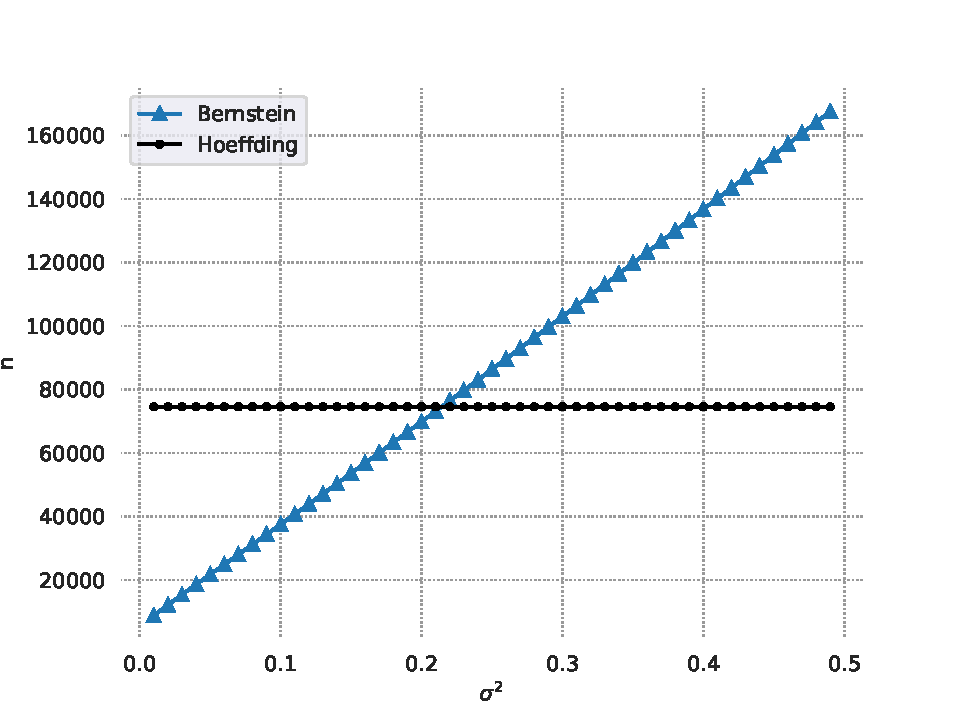
\includegraphics[width=0.75\textwidth]{imagens/t_eq_n.pdf}
		%latinmodern w pythonie
		\caption{Wykres maksymalnej potrzebnej ilości testów w zależności od wariancji zmiennych losowych  $X_i$ w przypadku gdy liczba testów jest równa liczbie gier ($t = n$) dla $\epsilon=0.01$ i $\delta = 0.05$.}
		\label{fig:t_eq_n}
	\end{figure}
	Z Rysunku \ref{fig:t_eq_n} widzimy zatem, że algorytm oparty o nierówność Bernsteina radzi sobie lepiej w przypadku gdy niskiej wariancji. Co więcej niezależnie od ilości wykonywanych testów, dla $\delta_n = \frac{0.05}{74540}$ maksymalna ilość gier po której z prawdopodobieństwem $1-0.05$ wiemy że $|\overline{X_i} - \mu| \le 0.01$ wynosi $74540$. Oznacza to że do Algorytmu \ref{alg:LEBR} możemy zastosować funkcje $\epsilon_k$ opartą o $\delta_k = \frac{\delta}{n_{max}}$ oraz dołożyć nowy warunek zatrzymania algorytmu gdy liczba wykonanych testów przekroczy $n_{max}$. Dotychczas uwzględnione poprawki przedstawione sa przy Algorytmu \ref{alg:ILEBR 1}.
	\begin{algorithm}[H]
		\caption{ILEBR 1}\label{alg:ILEBR 1}
		
		\begin{algorithmic}
			\Ensure precision $\epsilon$, probability $\delta$
			\State $LB \gets 0, \quad UB \gets \infty, \quad t \gets 0,\quad n \gets 1$
			\State Find $n_{max}$ such as $		\epsilon =  \sqrt{\frac{\ln(2n_{max}/\delta)}{2n_{max}}} $
			\Statex $\delta_n = \delta/n_{max}$
			\While{$ UB - LB > 2\epsilon $ or $n\le n_{max}$}  
			\State $t \gets t + 1$
			\State Obtain $X_t$
			\State $\epsilon_n \gets \overline{\sigma}_n \sqrt{\frac{2\ln(3/\delta_n)}{n}} + \frac{3  \ln{(3 / \delta_n)}}{n}$ 
			\State $LB \gets \max(LB,  \overline{X_n} - \epsilon_n)$
			\State $UB \gets \min(UB,  \overline{X_n} + \epsilon_n)$
			\State $n \gets n + 1$
			\EndWhile
			\State \Return $ \overline{X_t}$		
		\end{algorithmic}
	\end{algorithm}
	Algorytmy \ref{alg:LEBR} i \ref{alg:ILEBR 1} przeprowadzały testy po każdej rozegranej grzęz, skutkuje to wytopieniem bardzkiej ilości testów. Zamiast przeprowadzać test po każdej rozegranej grze, niech test odbywa się w momencie gdy liczba rozegranych gier będzie równa pewnej funkcji zależnej od ilości przeprowadzonych testów. Na podstawie artykuł \cite{heidrich2011non} wiemy że funkcja która pozwoli nam na polepszenie wyników jest $t = n^2$. Przeprowadźmy identyczną procedure jak w przypadku równań \eqref{eq:ILEBR Hoffdin} i \eqref{eq:ILEBR Bernstein}. Tym razem jednak zamiast stosować $t = n$ do Lematów \ref{Hoffding ineq lemma} i \ref{Bernsteina emp ineq lemma}  zastosujmy $t = n^2$.
	
	W przypadku granicy opartej o nierówność Hoffdina otrzymujemy
	\begin{gather}
		\label{eq:ILEBR Hoffdin t=n^2}
		\epsilon =  \sqrt{\frac{\ln(2n_{max}/\delta)}{2n_{max}^2}} \implies t_{max} = \lceil n_{max} \rceil^2 = \lceil213\rceil^2= 45369.
	\end{gather}
	W przypadku granicy opartej o nierówność Bernsteina otrzymujemy
	\begin{gather}
		\label{eq:ILEBR Bernstein t=n^2}
		0.01 \le \sqrt{\frac{\ln(\frac{3n_{max}}{0.05})}{n_{max}^2}} + \frac{3  \ln(\frac{3n_{max}}{0.05})}{n_{max}}^2\implies t_{max} = \lceil n_{max} \rceil^2 = \lceil230.751^2\rceil= 53247. 
	\end{gather}
	\begin{figure}
		\centering
		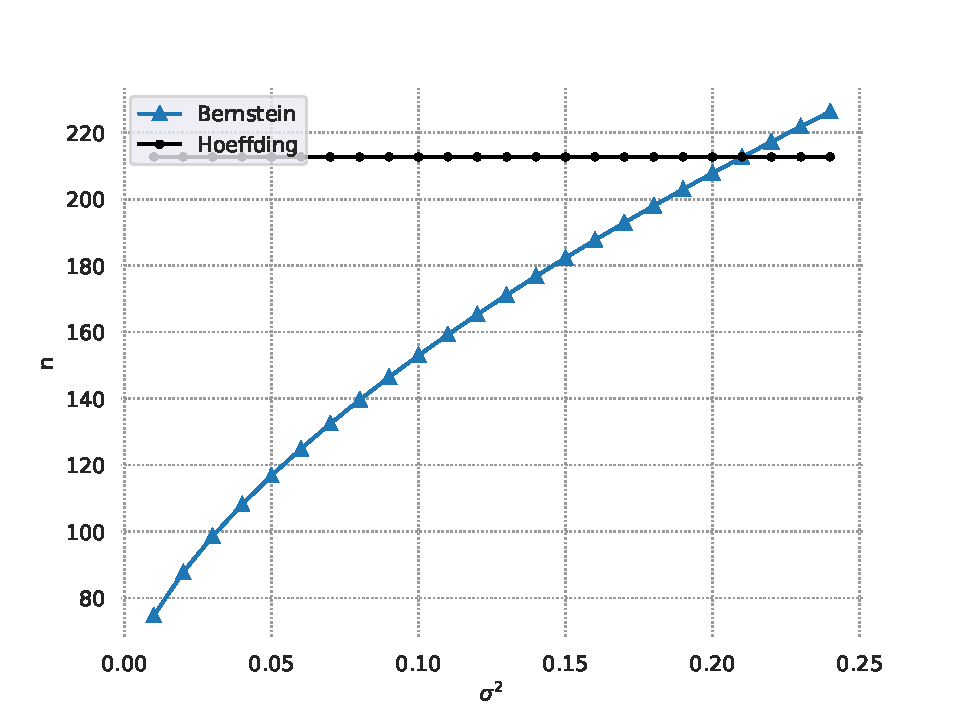
\includegraphics[width=0.8\textwidth]{imagens/t_eq_n_q.pdf}
%		\captionsetup{justification=centering}
		\caption{Wykres maksymalnej potrzebnej ilości testów w zależności od wariancji zmiennych losowych  $X_i$ w przypadku gdy liczba rozegranych gier jest równa liczbie przeprowadzonych testów do kwadratu ($t = n^2$) dla $\epsilon=0.01$ i $\delta = 0.05$.}
		\label{fig:t_eq_n_q}
	\end{figure}
	Porównując ze sobą uzyskane wartość z wzoru \eqref{eq:ILEBR Hoffdin} oraz \eqref{eq:ILEBR Hoffdin t=n^2} widzimy że udało się zmniejszyć maksymalną ilość gier jakie należny wykonać z 74540 do 45369.
	Wprowadźmy zatem nowo uzyskane poprawki trwożąc Algorytm \ref{alg:ILEBR 2}.
	\begin{algorithm}[H]
		\caption{ILEBR 2}\label{alg:ILEBR 2}
		\begin{algorithmic}
			\Ensure precision $\epsilon$, probability $\delta$
			\State $LB \gets 0, \quad UB \gets \infty, \quad t \gets 0,\quad n \gets 1$
			\State Find $n_{max}$ such as $		\epsilon =  \sqrt{\frac{\ln(2n_{max}/\delta)}{2n_{max}^2}} $
			\Statex $\delta_n = \delta/n_{max}$
			\While{$ UB - LB > 2\epsilon $ or $n \le n_{max}$}  
			\Repeat 
			\State $t \gets t + 1$
			\State Obtain $X_t$
			\Until $t=n^2$
			\State $\epsilon_n \gets \overline{\sigma}_n \sqrt{\frac{2\ln(3/\delta_n)}{n^2}} + \frac{3  \ln{(3 / \delta_n)}}{n^2}$ 
			\State $LB \gets \max(LB,  \overline{X_n} - \epsilon_n)$
			\State $UB \gets \min(UB,  \overline{X_n} + \epsilon_n)$
			\State $n \gets n + 1$
			\EndWhile
			\State \Return $ \overline{X_t}$		
		\end{algorithmic}
	\end{algorithm}
	Do tej pory Wszystkie stosowane algorytmy wyznaczały nam prawdopodobieństwo wygranej pierwszego gracza. Jednak nam nie zależny na tym dokładnie znać prawdopodobieństwo wygranej graczy. Głównym celem algorytmów jest odnalezienie lepszego gracza. Pozwala nam to modyfikacje Algorytmu \ref{alg:ILEBR 2} o nowe warunki zatrzymania.
	\begin{algorithm}[H]\captionsetup{labelformat=custom2}
		\caption{ILEBR* 1}\label{alg:IEBLR* 1}
		\begin{algorithmic}
			\Ensure precision $\epsilon$, probability $\delta$ 
			\State  $ LB \gets 0,\quad UB \gets \infty,\quad t \gets 1,\quad n \gets 0 $
			\State Find $n_{max}$ such as $		\epsilon =  \sqrt{\frac{\ln(2n_{max}/\delta)}{2n_{max}^2}} $
			\Statex $\delta_n = \delta/n_{max}$
			\While{$( UB - LB > 2\epsilon $ or $n < n_{max}+1)$ and $ (UB > 0.5 \text{ or } LB < 0.5)$}
			\Repeat 
			\State $t \gets t + 1$
			\State Obtain $X_t$
			\Until $t=n^2$
			\State $\epsilon_n \gets \overline{\sigma}_n \sqrt{\frac{2\ln(3/\delta_n)}{n^2}} + \frac{3  \ln{(3 / \delta_n)}}{n^2}$ 
			\State $LB \gets \max(LB,  \overline{X_n} - \epsilon_n)$
			\State $UB \gets \min(UB,  \overline{X_n} + \epsilon_n)$
			\State $n \gets n + 1$
			\EndWhile
			\If{$LB > 0.5$}
			\State \Return $p_1$ win
			\ElsIf{$UB < 0.5$}
			\State \Return $p_2$ win
			\ElsIf{$\overline{X_n} > 0.5$}
			\State \Return $p_1$ win
			\Else
			\State \Return $p_2$ win
			\EndIf
		\end{algorithmic}
	\end{algorithm}
	Do tej pory staraliśmy się ograniczyć z góry maksymalną ilość rozgrywanych gier. Jednak oczywistym faktem jest że nie ma sensu testowania który z graczy jest lepszy w monecie gdy ilość rozegranych gier jest niewystarczająco mały. Jadnak jak wyznaczyć nasze minimalne $t$ po którym zaczniemy testować? Algorytm oparte o nierówność Bernsteina najszybciej wyznaczają wynik w przypadku gdy wariancja naszej zmiennej losowej wynosi 0 (jeden z graczy zawsze wygrywa). Dla Algorytmu \ref{alg:IEBLR*} interesuje nas monet od którego będziemy w stanie rozróżnić kiedy dolna bać górna granica przekroczy $\frac{1}{2}$. Zatem oszacujmy $n_{min}$ korzystać z Lematu \ref{Bernsteina emp ineq lemma} dla $\overline{\sigma}_t=0$ i $t = n^2$.  
	
	
	
	\begin{gather*}
		\label{eq:ILEBR Bernstein t=n^2}
		0.5 \le \frac{3  \ln(\frac{3n_{max}}{0.05})}{n_{min^2}}\implies t_{min} = \lceil n_{min} \rceil^2 = \lceil7.53219\rceil^2= 64. 
	\end{gather*}
	Oznacza to, że przy $\epsilon=0.01$ i $\delta= 0.05$ w przypadku gdy jeden graczy wygrywa zawsze, będziemy w stanie to stwierdzić nie prędzej niż po 64 grach.
	Na tej podstawie wyznaczy nowe $n_{max}$ uwzględniając pomijanie pierwsze niepotrzebne testy.
	\begin{gather}
		\label{eq:ILEBR Hoffdin t=n^2 and t_min}
		0.01 =  \sqrt{\frac{\ln(2n_{max}/0.05)}{2(n_{max}+7)^2}} \implies t_{max} = \lceil n_{max}+6\rceil^2 = \left\lceil 205.289+7\right\rceil^2= 45369.
	\end{gather}
	Chociaż równanie \ref{eq:ILEBR Hoffdin t=n^2 and t_min} nie zmniejszyło nam maksymalnej liczby testów jakie należy wykonać to pozwoliło nam ono na zmniejszenie $\epsilon_n$. Oznacza to że stosują odroczenie pierwszych testów, pozwala nam na dokładniejsze oszacowanie naszej górnej i dolnej granicy w stosowanych algorytmach.
	\begin{algorithm}[H]\captionsetup{labelformat=custom2}
		\caption{ILEBR* 2}\label{alg:IEBLR* 2}
		\begin{algorithmic}
			\Ensure precision $\epsilon$, probability $\delta$ 
			\State  $ LB \gets 0,\quad UB \gets \infty, \quad n \gets 0 $
			\State Find $n_{max}$ such as $		\epsilon =  \sqrt{\frac{\ln(2n_{max}/\delta)}{2n_{max}^2}} $
			\State Find $n_{min}$ such as $		0.5 =  \sqrt{\frac{\ln(2n_{max}/\delta)}{2(n_{min}+1)^2}} $
			\State Obtain first $X_1,X_2,X_{n_{min}}$ games 
			\State $t \gets n_{min}^2$
			\Statex $\delta_n = \delta/n_{max}$
			\While{$( UB - LB > 2\epsilon $ or $n \le n_{max})$ and $ (UB > 0.5 \text{ or } LB < 0.5)$}
			\Repeat 
			\State $t \gets t + 1$
			\State Obtain $X_t$
			\Until $t=n^2$
			\State $\epsilon_n \gets \overline{\sigma}_n \sqrt{\frac{2\ln(3/\delta_n)}{(n+n_{min})^2}} + \frac{3  \ln{(3 / \delta_n)}}{(n+n_{min})^2}$ 
			\State $LB \gets \max(LB,  \overline{X_n} - \epsilon_n)$
			\State $UB \gets \min(UB,  \overline{X_n} + \epsilon_n)$
			\State $n \gets n + 1$
			\EndWhile
			\If{$LB > 0.5$}
			\State \Return $p_1$ win
			\ElsIf{$UB < 0.5$}
			\State \Return $p_2$ win
			\ElsIf{$\overline{X_n} > 0.5$}
			\State \Return $p_1$ win
			\Else
			\State \Return $p_2$ win
			\EndIf
		\end{algorithmic}
	\end{algorithm}
	\section{Moc testów statysytycznych}
	Mocą testu statystycznego nazywamy prawdopodobienstwo unikniecia popełnenia błędu drugiego rodzaju, czyli prawdopoodbienstwo przyjecie hipotezy zerowej gdy w rzeczywistosci jest ona fałszywa. W naszym przypadku jest to prawdopodobienstwo przyjecia za lepszego gracza osoby o niższym prawdopodobienstiwe wygranej.
	Wysoka moc testu jest pożadaną własciwoscia testu, jednak żadanie jaknajlepszej mocy może wiazać się z zwiększeniem próby badawczej.
	
	%zamiast pisac test statystyczny uzywac problem decyzyjny
	%zamiast mocy prawdopodobienstwo błędu
	\begin{figure}
		\centering
		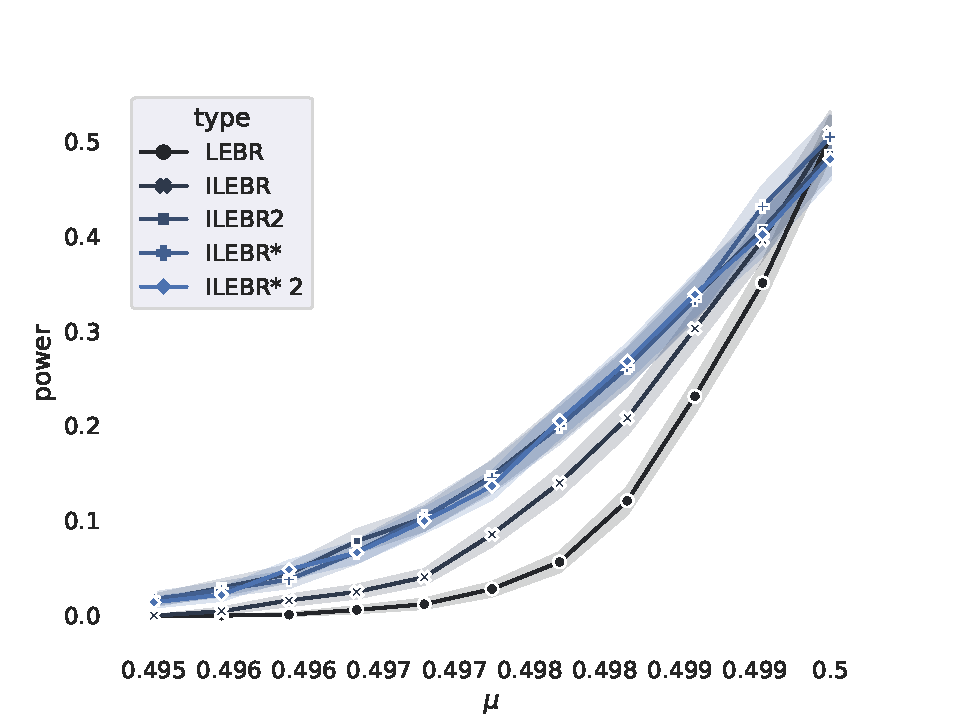
\includegraphics[width=0.7\textwidth]{imagens/test_powrs.pdf}
		\caption{Wykres mocy testów statystycznych w zależności od wartosci oczekiwanej zmiennych losowych  $X_i$ dla $\epsilon=0.01$ i $\delta = 0.05$.}
		\label{fig:test_powrs}
	\end{figure}
	\begin{figure}
		\centering
		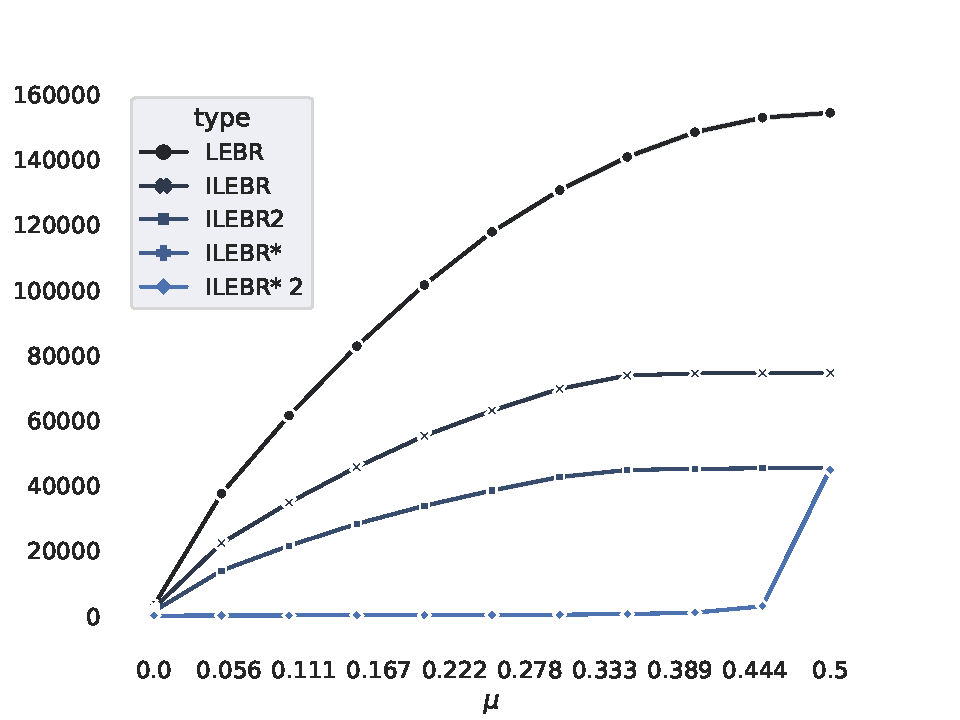
\includegraphics[width=0.7\textwidth]{imagens/needed_games_to_play.pdf}
		\caption{Wykres sredniej liczby gier potrzebej do rozegrania w zależności od wartosci oczekiwanej zmiennych losowych  $X_i$ dla $\epsilon=0.01$ i $\delta = 0.05$.}
		\label{fig:needed_games_to_play}
	\end{figure}
	Patrząc wyłączanie na Rysunek \ref{fig:test_powrs} możemy zobaczyć że wszystkie testu czują się dobrą mocą i działają bardzo dobrze do memento gdy jeden z graczy ma prawdopodobieństwo wygranej bliskie 0.495. Dodatkowo obszary ściemnione oznaczają 95\% przedziały ufności.
	
	
	Porównując ze sobą wyniki przedstawione na Rysunkach \ref{fig:test_powrs} i \ref{fig:needed_games_to_play} możemy stwierdzić, że testem o
	najlepszej mocy jest testo oparty o algorytm LEBR, jednak wymaga on bardo dłużej liczby gier potrzebnych do rozegrania.
	Test statystyczny oparty o algorytm ILEBR ma gorsza moc ale pozwala nam na prawie dwukrotnie zmniejszenie liczby wymaganych gier. Dodatkowo widzimy że algorytmy  ILEBR 2, ILEBR* i ILEBR* 2 cechują się mocą na bardzo podobnym poziomie jednak wersje algorytmy oznaczone * pozwalają nam bardo duże ograniczenie liczby gier potrzebnej do rozegrania aby test mógł wyznaczyć lepszego gracza. W poniższej pracy będziemy stosować algorytm ILEBR* 2 ponieważ pozwoli on na znacznie niezwieszenie liczby porównań jakie będziemy przeprowadzacz w celu wyznaczenia lepszego gracza. 
	
	\section{Algorytmy wyznaczania optymalnej strategi}
	Wszystkie algorytmy przedstawione w tym rozdziale są algorytmami genetycznymi \cite{Figielska2006}. 
	Algorytm generacyjny to sposób tworzenia nowych rozwiązań dla danego problemu poprzez iteracyjne stosowanie procesu ewolucyjnego. W tym procesie tworzone są nowe rozwiązania, oceniane ich jakość i wybierane najlepsze z nich, aby stworzyć kolejną generację rozwiązań. Ten proces powtarza się, aż zostanie znalezione rozwiązanie spełniające określone kryteria. Algorytm generacyjny może być używany do rozwiązywania różnych rodzajów problemów, takich jak optymalizacja, uczenie maszynowe, tworzenie sztucznej inteligencji i wiele innych. Algorytmy ewolucyjne są często interpretowane jako odwzorowanie procesu ewolucyjnego w naturze, ze względu na swoje odpodobnienie do procesu selekcji naturalnej w którym najlepsze jednostki są wybierane do reprodukcji i tworzenia nowych pokoleń.
	
	Ogólnie rzecz biorąc, algorytm generacyjny składa się z kilku kluczowych kroków:
	\begin{itemize}
		\item Inicjalizacja: Tworzenie początkowej zbioru rozwiązań dla danego problemu.
		\item Ocena: Ocena jakości każdego z rozwiązań za pomocą odpowiedniej funkcji celu lub innych miar.
		\item Selekcja: Wybieranie najlepszych rozwiązań do następnej generacji.
		\item Krzyżowanie: Łączenie najlepszych rozwiązań z poprzedniej generacji, aby stworzyć nowe rozwiązania dla następnej generacji.
		\item Mutacja: Losowa zmiana jednego lub więcej elementów w nowych rozwiązaniach, aby zapewnić różnorodność w następnej generacji.
		\item Powtarzanie: Powtarzanie kroków 2-5, aż zostanie znalezione rozwiązanie spełniające określone kryteria jakości lub osiągnięty zostanie maksymalny poziom iteracji.
	\end{itemize}	
	Proces znajdowania potencjalnych rozwiązań polega na przeszukiwaniu przestrzeni wszystkich możliwych rozwiązań i wybieraniu tych, które dają najlepsze wyniki. W rzeczywistości jednak często nie mamy fizycznej możliwości sprawdzenia wszystkich możliwych rozwiązań lub ich sprawdzenie jest zbyt czasochłonne lub kosztowne. Dlatego w algorytmach ewolucyjnych często wykorzystuje się techniki probabilistyczne, które pomagają wybierać, tworzyć i wyszukiwać kolejne rozwiązania.
	
	W niniejszej pracy zaprezentujemy 4 algorytmy, których celem jest znalezienie optymalnej strategii. Trzy pierwsze algorytmy zostaną opisane na podstawie pracy \cite{cauwet2018surprising}]. Czwartym algorytmem jest proponowana przeze mnie metoda, która jest bardzo podobna do algorytmu trzeciego (patrz [referencja]). Opis tego algorytmu zostanie przedstawiony w dalszej części pracy.

	\subsection{Argorytm itereacyjny}
		Pierwszym algorytmem, który zostanie przedstawiony, jest algorytm iteracyjny. Jest to metoda bardzo intuicyjna, opierająca się na stopniowym zwiększaniu skuteczności strategii graczy poprzez porównywanie ich wyników. Gdy znajdziemy strategię, która daje lepsze wyniki niż ta poprzednia, staje się ona nowym punktem odniesienia (baseline). W oparciu o tę nową strategię algorytm będzie kontynuować proces optymalizacji wyników graczy. Nowa strategia jest akceptowana, jeśli wygrywa ona z prawdopodobieństwem większym niż 50\% w porównaniu do poprzedniej strategii. Algorytm \ref{alg:Iterative} jest przykładem algorytmem ewolucyjnym typu (1+1) \cite{droste1998rigorous}.
		\begin{algorithm}\captionsetup{labelformat=custom2}
			\caption{Iterative algorithm}\label{alg:Iterative}
			\begin{algorithmic}
				\Ensure  precision $\epsilon$, probability $\delta$, random opponent $x$
				\State $\sigma \gets 1 $ \Comment{Inital step-size}
				\While{(termination criterion is not met)}
				\ForAll{$i = 1$ to lenght of x}
				\State $x_i' \gets x_i + \sigma \mathcal{N}(0,1)$ \Comment{Mutation}
				\EndFor
				\Repeat
				\State play game between $x'$ and $x$
				\Until{the limited Bernstein race of precision $\epsilon$ stop}
				\If{$x'$  better then $x$  }
				\State $x \gets x'$
				\State $\sigma \gets 1.25\sigma$
				\Else
				\State $\sigma \gets 0.84 \sigma$
				\EndIf
				\EndWhile
				\State \Return an approximation x of the optimal strategy
			\end{algorithmic}
		\end{algorithm}

	\subsection{Real Coevolution algorytm}	
	Kolejnym algorytmem ewolucyjnym, którego będziemy używać, jest algorytm koewolucyjny. W przypadku tej metody nowy punkt odniesienia jest wybierany w momencie, gdy nowo znaleziona strategia okazuje się lepsza niż wszystkie dotychczas wybrane strategie. Pseudokod algorytmu koewolucyjnego został przedstawiony jako Algorytm \ref{alg:Coevolution}. 

	\begin{algorithm}\captionsetup{labelformat=custom2}
		\caption{Real Coevolution}\label{alg:Coevolution}
		\begin{algorithmic}
			\Ensure  precision $\epsilon$, probability $\delta$, random opponent $x$
			\State $\sigma \gets 1 $ \Comment{Inital step-size}
			\State $P \gets \{ x \}$ \Comment{Best point population}
			\While{(termination criterion is not met)}
			\ForAll{$i = 1$ to lenght of $x$}
			\State $x_i' \gets x_i + \sigma \mathcal{N}(0,1)$ \Comment{Mutation}
			\EndFor
			\ForAll{$i = 1$ to lenght of $P$}
			\Repeat
			\State play game between $x'$ and $P_i$
			\Until{each limited Bernstein race of precision $\epsilon$ stops}
			\EndFor
			\If{$x'$  better then all points in $P$}
			\State $x \gets x'$
			\State $P \gets \{P,x'\}$
			\State $\sigma \gets 1.25\sigma$
			\Else
			\State $\sigma \gets 0.84 \sigma$
			\EndIf
			\EndWhile
			\State \Return an approximation x of the optimal strategy
		\end{algorithmic}
	\end{algorithm}

	\subsection{Aproxx Coevolution 1 algorytm}
	W przypadku dwóch poprzednich algorytmów nowe rozwiązanie jest tworzone na podstawie poprzednio znalezionego rozwiązania. Możemy jednak zastosować tzw. ''podejście Paryskie'' (Parisian approach). W tym podejściu zamiast porównywać nowo uzyskaną strategię z każdą poprzednio przyjętą, porównujemy ją tylko z jedną losowo wybraną strategią z populacji. Pseudokod algorytmu koewolucyjnego został przedstawiony jako Algorytm \ref{alg:Approximate_Coevolution}. 
	\begin{algorithm}\captionsetup{labelformat=custom2}
		\caption{Approximate Coevolution}\label{alg:Approximate_Coevolution}
		\begin{algorithmic}
			\Ensure  precision $\epsilon$, probability $\delta$, random opponent $x$
			\State $\sigma \gets 1 $ \Comment{Inital step-size}
			\State $P \gets \{ x \}$ \Comment{Best point population}
			\While{(termination criterion is not met)}
			\ForAll{$i = 1$ to lenght of $x$}
			\State $x_i' \gets x_i + \sigma \mathcal{N}(0,1)$ \Comment{Mutation}
			\EndFor
			\Statex \ \ \ \ Draw at random an integer $rand$ between 1 and the size of $P$
			\Repeat
			\State play game between $x'$ and $rand^\text{th}$ individual of P
			\Until{each limited Bernstein race of precision $\epsilon$ stops}
			\If{$x'$  better then all points in $P$}
			\State $x \gets x'$
			\State $P \gets \{P,x'\}$
			\State $\sigma \gets 1.25\sigma$
			\Else
			\State $\sigma \gets 0.84 \sigma$
			\EndIf
			\EndWhile
			\State \Return an approximation x of the optimal strategy
		\end{algorithmic}
	\end{algorithm}
	
	\subsection{Aproxx Coevolution 2 algorytm}
	Ostatnim algorytmem, którym się zajmiemy, jest kolejny algorytm koewolucyjny. Tym razem, zamiast porównywać naszą strategię z jedną losowo wybraną strategią z populacji, tak jak to robiliśmy w przypadku Algorytmu \ref{alg:Approximate_Coevolution}, nasza strategia będzie testowana przeciwko losowo wybranemu przeciwnikowi.Pseudokod algorytmu koewolucyjnego został przedstawiony jako Algorytm \ref{alg:Approximate_Coevolution_2}. 

	\begin{algorithm}\captionsetup{labelformat=custom2}
		\caption{Approximate Coevolution 2}\label{alg:Approximate_Coevolution_2}
		\begin{algorithmic}
			\Ensure  precision $\epsilon$, probability $\delta$, random opponent $x$
			\State $\sigma \gets 1 $ \Comment{Inital step-size}
			\State $P \gets \{ x \}$ \Comment{Best point population}
			\While{(termination criterion is not met)}
			\ForAll{$i = 1$ to lenght of $x$}
			\State $x_i' \gets x_i + \sigma \mathcal{N}(0,1)$ \Comment{Mutation}
			\EndFor
			\Repeat {\ play game between $x'$ and random individual of P}
			\Until{each limited Bernstein race of precision $\epsilon$ stops}
			\If{$x'$  better then all points in $P$}
			\State $x \gets x'$
			\State $P \gets {P,x'}$
			\State $\sigma \gets 2\sigma$
			\Else
			\State $\sigma \gets 0.84 \sigma$
			\EndIf
			\EndWhile
			\State \Return an approximation x of the optimal strategy
		\end{algorithmic}
	\end{algorithm}
	
	\chapter{Gry}
	"Aby sprawdzić poprawność działania powyższych algorytmów, przetestujemy je na podstawie dwóch gier. Pierwszą z nich będzie popularna gra karciana zwana Wojną. Drugą grą, w której będziemy szukać optymalnej strategii, będzie gra o nazwie Rrrats. Przedstawmy najpierw zasady obowiązujące w obu tych grach.

	\section{Gra w wojnę}
	Wojna to prosta gra karciana, w której uczestnicy grają przeciwko sobie i używają talii standardowych kart do gry. Celem gry jest zdobycie wszystkich kart od przeciwnika.
	
	Zasady gry są następujące:
	\begin{itemize}
		\item 	Gracze rozdają po 26 kart, tak aby każdy miał swoje ukryty "magazyny".
		
		\item Następnie jedna karta jest odkrywana z każdego magazynu i porównywana ze sobą. Gracz, który ma kartę o wyższej wartości, zabiera obie karty i dokłada je na koniec swojego magazynu. Jeśli karty są takie same, gracze rozgrywają "wojnę".
		
		\item W przy wojny, oboje gracze wykładają z magazynów najpierw jedną kartę rewersem do góry, a następnie odkrywają kolejną kartę rewersem do dołu. Ten gracz, który ma kartę o wyższej wartości, zabiera wszystkie karty i dokłada je do swojego magazynu. Jeśli karty są takie same, proces powtarza się, aż do momentu gdy jeden z graczy wygra.
		
		\item Gra kończy się w monecie któryś z graczy wygra wszystkie karty.
	\end{itemize}
	Same zasady gry nie definiują jednak tego w jaki sposób karty na koniec naszego "magazynu" mogą zostać umieszczane.
	
	Wprowadźmy zatem 3 parametry nazwijmy je odpowiednio $A,\:B,\:C$, których będziemy używać do wyznaczania nieujemnych parametrów $\alpha = \exp(A),\: \
	\beta= \exp(B),\: \gamma= \exp(C)$. Wtedy, umieśćmy $k$ wygranych kart na końcu naszego "magazynu" niestepujący sposób:
	\begin{itemize}
		\item karty w kolejności malejącej z prawdopodobieństwem równym $\alpha/(\alpha+\beta+\gamma)$ 
		
		\item karty w kolejności rosnącej z prawdopodobieństwem równym $\beta/(\alpha+\beta+\gamma)$ 
		
		\item karty w kolejności losowej z prawdopodobieństwem równym $\gamma/(\alpha+\beta+\gamma)$ 
	\end{itemize}
	
	\section{Rrrats!}
	Rrrats jest prosta grą kościaną typu ekstensywnego, a jej celem jest zdobycie przez poszczególnego gracza najwierniejszej liczby punktów. W każdej swojej turze gracz rzuca dwiema takomskim, aż do momentu gdy zostanie spełniony warunek stopu, bądź sam uzna że nie chce już konturować. Gra kończy się w momencie gdy z głównego stosu znikną wszystkie 31 żetonów (punktów). W grze ożywa się specjalnych których prawdopodobieństw uzyskania otwarci $0,\:1,\:2$ wynosi odnowienie $3/6,\:2/6,\:1/6$.
	
	Zasady gry sa następujące:
	\begin{itemize}[]
		\item Grac w swojej turze może rzucić dwoma kosterskimi dowolną ilość razy
		\item  Gracz wykonuje następujące akcje w zależności od uzyskanego wyniku:
		\begin{enumerate}
			\item[a)] Jeśli na kostce wypadło 1, gracz bierze do "reki" żeton z stosu głównego.
			\item[b)] Jeśli wypadło 2, gracz kranie punkt przeciwnikowi i bierze go do swojej "reki". Jeśli to nie możliwe gracz bierze punkt z stosu głównego. 
			\item[c)] Jeśli upadło 0, nic się nie dzieje.
			\item[d)] Jeśli na obu kostkach wypadło 0, gracz kończy swoją turę i odkłada wszystkie punkty jakie ma w "ręce".
			\begin{description}
				\item[Przykład:] Jeśli na kostkach wypadnie 0 i 1 gracz pobiera 1 punkt ze stosu głowniowe. Jeśli an kostkach wypadnie 1 i 1 gracz pobiera 2 punkty ze stosu głównego. 
			\end{description}		
		\end{enumerate}
		\item Po każdym żucie gracz decyduje się na to czy grac dalej, czy zakończyć swoja torę.
		
		\item Jeśli gracz ma więcej niż 4 punktów w "rece" tura gracza automatycznie się kończy a uzyskaną nadwyżkę odkłada się do stosu głównego.
		
		\item Jeśli tura dobiegła końca, to gracz przenośni wszystkie punkty uzyskane na "ręce" do swojej puli puntów osobistych.
		
		\item Gra kończy się w momencie gdy liczba punktów na głowy stosie wyniesie 0.
	\end{itemize}

		W tym przypadku strategia której będziemy szukać będzie oparta o 8 parametrów $A_1,\: A_2, B_1,\: B_2, C_1,\: C_2, D_1,\: D_2$. Przy pomocy tych paramentów wyznaczymy kolejne 8 współczynników 
		$
		\alpha_1 = \exp(A_1),\:
		\alpha_2 = \exp(A_2), 
		\beta_1= \exp(B_1),\: 
		\beta_2= \exp(B_2), 
		\gamma_1= \exp(C_1),\: 
		\gamma_2= \exp(C_2)
		$. Naszym celem jest wyznaczenie prawdopodobieństwa zdecydowania się na dalszy rzut kośćmi w zależność od ilości punktów posiadanych na "ręce". Wprowadźmy zatem  zmienna losowa $Y|K=k,\: k=\{1, 2, 3\}$. Posłuży ona  nam do wyznaczenia prawdopodobieństwo zdecydował się na dalszy rzut kośćmi ($Y=1$) w zależności od ilości posiadanych punktów na "rece". 
		
		Same prawdopodobieństwa wprowadzonej ziemnej losowej określamy w następujący sposób:  
		\begin{gather*}
			 P(Y = 1|K=1) = \alpha_1/(\alpha_1+\alpha_2),\\
			 P(Y = 1|K=2) = \beta_1/(\beta_1+\beta_2),\\
			 P(Y = 1|K=3) = \gamma_1/(\gamma_1+\gamma_2). 
		\end{gather*}


	
	\chapter{Wyniki}
	Do przedstawienia wyników dziania przedstawionych algorytmów ożyjemy dwóch. Pierwsza z nich będzie tabela obrazująca prawdopodobieństwo granej strategi uzyskanych przez jazdy z algorytmów przeciwko strategi pocztowej. Droga tabele zobrazuje natomiast wyniki działania naszych strategii przeciwko strategią uzyskanym przez pozostałe algorytmy.
	Wyniki przedstawione na Tabelach \ref{table:war_results} i \ref{table:rrrats_results} oraz Rysunkach \ref{fig:war_results} i \ref{fig:rrrats_results} pokakują, że kazdemu z naszych alkorytmów odało sie zdaleśc strategie dającą sredio wikszy winnik od losowej strategi poczatkowej. Dodatkowo wyzaczone straetegie możemy zinterpretowac interpretować wprosty do zlozymnienia dla człowieka sposób.
	W grze wojnnie istnieje strategia prosta, jest nią ukłądanie kart zawse w kolejnosci od nawiekszej do najmniejszej. Dodatkowo strategia ta ma 70\% szans na wygranie przeciwko straetgi ukłądania kart w sposób malejaćy, oraz 53\% szans na wygranie przeciwko strategi losowej.
	\begin{table}[h]
		\begin{center}
			\begin{tabular}{lrrrr}
				\toprule
				{} &  iterawtive &  coevolution &  approx coevolution &  approx coevolution 2 \\
				\midrule
				mean  &    0.541617 &     0.545225 &             0.530655 &               0.528750 \\
				std   &    0.005623 &     0.005158 &             0.004900 &               0.005244 \\
				min   &    0.525300 &     0.532900 &             0.517400 &               0.514000 \\
				25\%   &    0.538300 &     0.541100 &             0.527600 &               0.525800 \\
				50\%   &    0.540600 &     0.544600 &             0.530600 &               0.529200 \\
				75\%   &    0.545575 &     0.548800 &             0.534700 &               0.532500 \\
				max   &    0.556100 &     0.556700 &             0.542200 &               0.540100 \\
				\bottomrule
			\end{tabular}
			\caption{Rezultaty uzyskanych strategi przeciwko strategi poczatkowej dla gry Rrrats!.}
			\label{table:war_results}
		\end{center}
	\end{table}
	\begin{table}[h]
		\begin{center}
			\begin{tabular}{lrrrr}
				\toprule
				{} &  iterawtive &  coevolution &  approx coevolution &  approx coevolution 2 \\
				\midrule
				mean  &    0.786629 &     0.780805 &             0.787310 &               0.759073 \\
				std   &    0.003581 &     0.004265 &             0.003586 &               0.004170 \\
				min   &    0.778600 &     0.768400 &             0.778500 &               0.748300 \\
				25\%   &    0.784550 &     0.777925 &             0.785575 &               0.756525 \\
				50\%   &    0.786600 &     0.780700 &             0.787350 &               0.758700 \\
				75\%   &    0.788800 &     0.783300 &             0.789125 &               0.761500 \\
				max   &    0.798400 &     0.789700 &             0.796700 &               0.772200 \\
				\bottomrule
			\end{tabular}
			\caption{Rezultaty uzyskanych strategi przeciwko strategi poczatkowej dla gry Wojna.}
			\label{table:rrrats_results}
		\end{center}
	\end{table}
	
	\begin{figure}
		\centering
		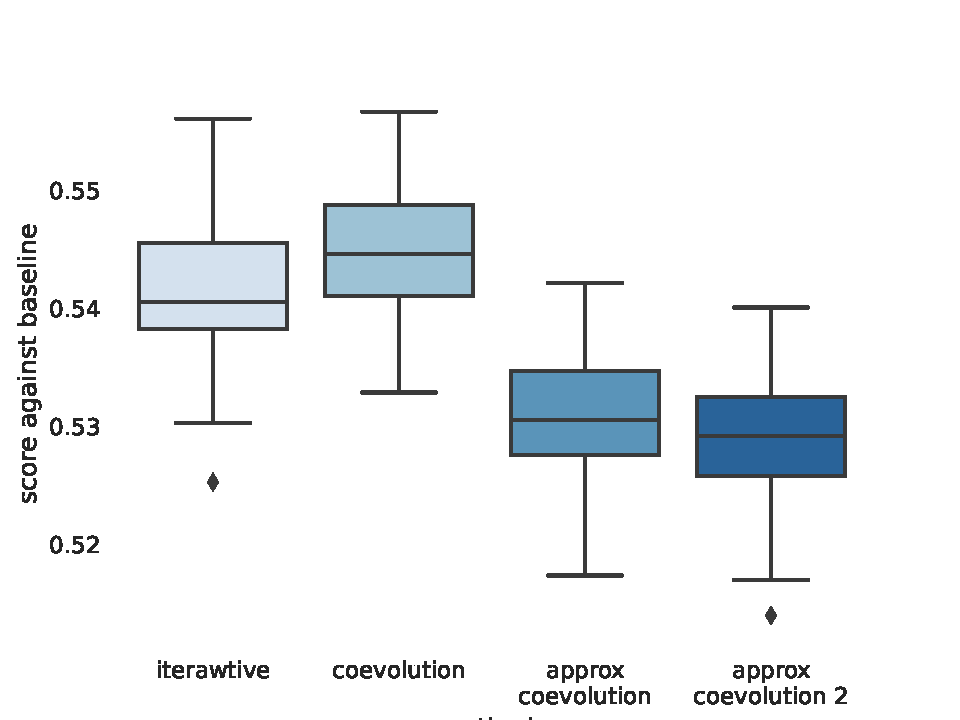
\includegraphics[width=0.8\textwidth]{imagens/war_results.pdf}
		%latinmodern w pythonie
		\caption{Wykresy pódełkowe przedwaiajace rezultaty uzyskanych strategi przeciwko strategi poczatkowej dla gry Wojna.}
		\label{fig:war_results}
	\end{figure}
	\begin{figure}z
		\centering
		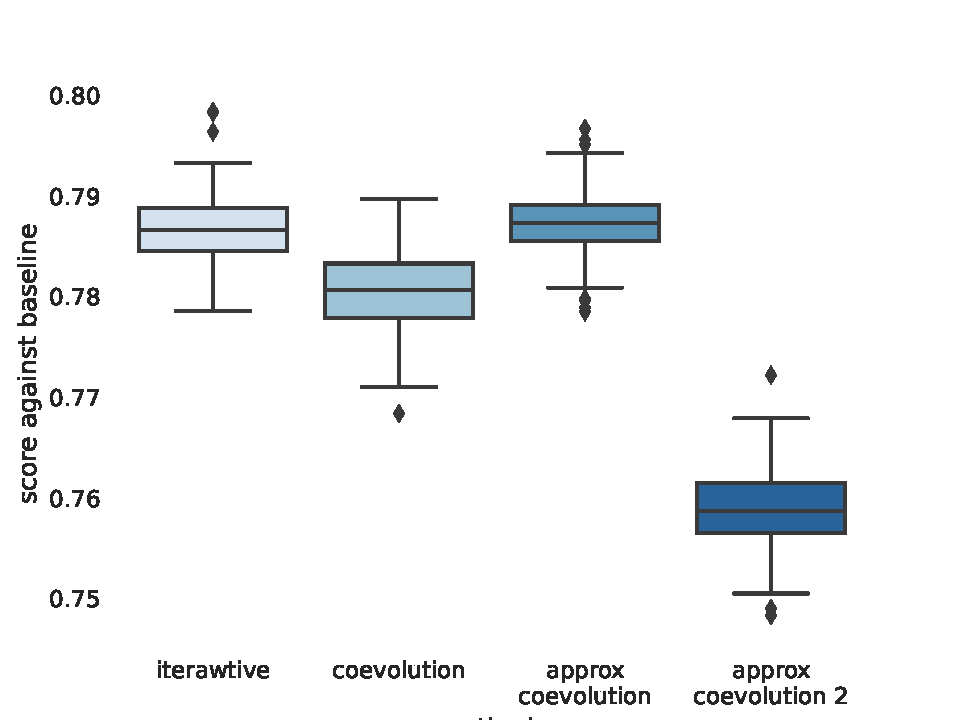
\includegraphics[width=0.8\textwidth]{imagens/rrrats_results.pdf}
		%latinmodern w pythonie
		\caption{Wykresy pódełkowe przedwaiajace rezultaty uzyskanych strategi przeciwko strategi poczatkowej dla gry Rrrats.}
		\label{fig:rrrats_results}
	\end{figure}
	
	


	\newpage
	\section{ernstein race without maximum race length}
	Wykorzystując Lemat~\ref{Bernsteina emp ineq lemma} oraz korektę \ref{korekta 2} z $\delta_k=\frac{c\delta}{k^2}, c=\frac{6}{\pi^2}$ otrzymujemy, że dla ciągu $X_1,X_2,\dots,X_t$ i.i.d. zmiennych losowych takim, że  $0 \le X_i \le 1$ 
	\begin{align*}
		\label{Bernstein race without maximum race length}
		\epsilon_{t,k} \le \overline{\sigma}_t \sqrt{\frac{2\ln(3/\delta_k)}{t}} + \frac{3  \ln{(3 / \delta_k)}}{t} =
		\overline{\sigma}_t\sqrt{\frac{2\ln(\frac{k^2\pi^2}{2\delta})}{t}} + \frac{3  \ln{(\frac{k^2\pi^2}{2\delta})}}{t}
	\end{align*}
	Wtedy $e_{t,k}$ interpretujemy jako maksymalną różnicę między empiryczną a teoretyczną wartością oczekiwaną po przeprowadzeniu $k$ testów i rozegraniu $t$ gier, z prawdopodobieństwem pomyłki równym 
	\begin{lemma}
		\label{lemma Bernstein race without maximum race length}
		Niech liczba rozegranych gier będzie funkcja zależną od k ($f(k) = t$) oraz niech $\delta_k = \frac{\delta}{g(k)}$
		gdzie $\delta \ge \sum_{k=1}^{\infty} \frac{\delta}{g(k)}$ i $\ln(g(k)) \in o(f(k))$. Wtedy
		$\lim\limits_{k\to\infty} e_{f(k),k} = 0$ 
	\end{lemma}
	\begin{proof}[Dowód Faktu \ref{lemma Bernstein race without maximum race length}]
		\begin{gather*}
			0\le X_i \le 1 \implies \overline{\sigma}_t^2 \le \frac{1}{2}\\
			\epsilon_{f(k), k} \le  \sqrt{\frac{\ln(\frac{3g(k)}{\delta})}{f(k)}} + \frac{3  \ln{(\frac{3g(k)}{\delta})}}{f(k)}
		\end{gather*}
		Z założeń wiemy ze $ln(g(k)) \in o(f(k))$, zatem
		\begin{gather*}
			\lim\limits_{k\to\infty} \frac{  \ln{(\frac{3f(k)}{\delta})}}{f(k)} = 0
		\end{gather*}
		Co ostatecznie z tw. o trzech ciągach daje nam
		\begin{gather*}
			0\le \lim\limits_{k\to\infty} e_{f(k), k} \le 0 \implies \lim\limits_{t\to\infty} e_{f(k), k} = 0
		\end{gather*}
	\end{proof}
	Lemat \ref{lemma Bernstein race without maximum race length} pozwala nam na to aby ograniczyć ilość przeprowadzanych testów. Ponieważ podejście oparte o testowane który z graczy jest lepszy po każdej rozegranej grze prowadzi do nadmiarowej ilości wykonywanych testów.
	Przykładem funkcjami jakimi użyć do Lematu \ref{lemma Bernstein race without maximum race length} są $f(k) = k^2,\; g(k) = \frac{6/\pi^2}{k^2}$. Teaki dobór funkcji oznacza ze $k$-ty test odbywa się gdy liczba przeprowadzonych gier wynosi $k^2$.
	

	
	
{\backmatter \chapter{Podsumowanie}}
Podsumowanie w pracach matematycznych nie jest obligatoryjne. Warto jednak na zakończenie krótko napisać, co udało nam się zrobić w pracy, a czasem także o tym, czego nie udało się zrobić.

{\backmatter \chapter{Dodatek}}
Dodatek w pracach matematycznych również nie jest wymagany. Można w nim przedstawić np. jakiś dłuższy dowód, który z pewnych przyczyn pominęliśmy we właściwej części pracy lub (np. w przypadku prac statystycznych) umieścić dane, które analizowaliśmy.

%%%%%%%%%%%%%%%%%%%%%%%%%%%%%%%%%%%%%%%%%%%%%%%%%%%%%%%%%
% BIBLIOGRAFIA5
% W tworzeniu bibliografii najlepiej korzystać z BibTex'a, 
% który jest częścią systemu Tex. W naszym przypadku funkcję 
% przechowalni literatury, do której się odwołujemy, pełni 
% plik bibliografia.bib. Nie musimy ręcznie dodawać nowych 
% pozycji do bibliografii. Możemy wejść np. na stronę 
% https://mathscinet.ams.org/mathscinet/index.html, 
% znaleźć odpowiednią pozycję, wybrać ją, a następnie zmienić 
% 'Select alternative format' na BibTeX, skopiować uzyskany 
% tekst, wkleić do pliku bibliografia.bib i skompilować. 
% Gotowe informacje do pliku bibliografia.bib można znaleźć 
% także na https://arxiv.org - gdy znajdziemy interesującą nas 
% pracę, szukamy 'References & Citations' i klikamy 'NASA ADS', 
% a potem 'Bibtex entry for this abstract' 
% i postępujemy tak jak wcześniej.
%%%%%%%%%%%%%%%%%%%%%%%%%%%%%%%%%%%%%%%%%%%%%%%%%%%%%%%%%
\newpage
% w nawiasie klamrowym wpisujemy nazwę pliku z bibliografią w formacie .bib

\bibliographystyle{bibliografia_styl}
\bibliography{bibliografia}
\end{document}